\documentclass[12pt]{article}
\usepackage{graphicx}
\usepackage{caption}
\usepackage{subcaption}
\usepackage{tikz}
\usepackage{venndiagram}
\usepackage{venndiagram}
\usepackage{tcolorbox}
\usepackage{listings}
\usepackage{enumitem}
\usepackage{amsmath}
\usepackage{amssymb}
\usepackage{colortbl}
\usepackage{xcolor}
\usepackage[margin=1cm, top=1.5cm, bottom=1.5cm]{geometry}

\tcbuselibrary{breakable}

\title{\textbf{Gráficas y Juegos: Tarea 02}}
\author{Larios Ponce Hector Manuel\\Rendón Ávila Jesús Mateo\\Valencia Morales Indra Gabriel }
\date{\today}

\begin{document}

\maketitle
\begin{center}
\vspace{3cm}
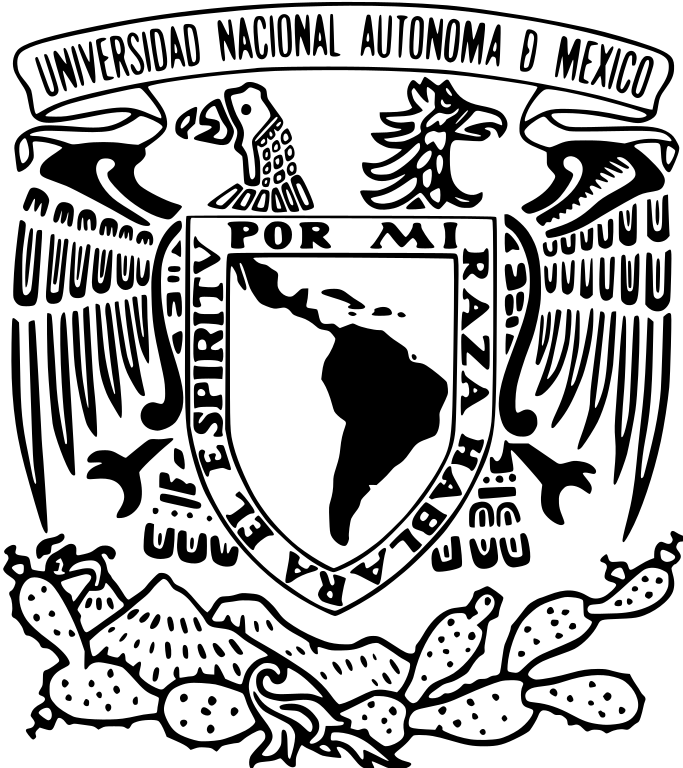
\includegraphics[width=0.195\textwidth]{Escudo.png}
\hspace{0.5cm}
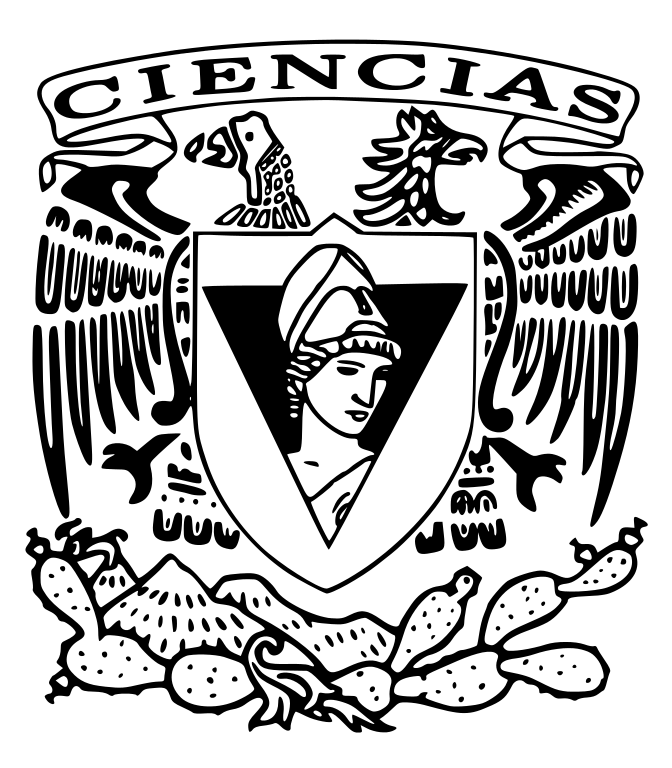
\includegraphics[width=0.2\textwidth]{logo_ciencias.png}
\end{center}
\begin{center}
    \vspace{1cm}
    Universidad Nacional Autónoma de México\\
    Facultad de Ciencias\\
    Profesor: César Hernández Cruz\\
\end{center}

\newpage

%
% Ejercicio 1
%
\textbf{1.} Sea $(R, +, \ast)$ un anillo. Demostrar mediante definiciones que $R$ es conmutativo si y sólo si
$\forall x, y, \in R$ se cumple: $(x + y) \ast (x - y) = x^2 - y^2$\\

$\Longrightarrow)$ $Hipotesis$. R es conmutativo.\\

$P.D$. Bajo la operaicón de la operación del producto se cumple que $\forall x, y \in R$ $(x + y) \ast (x - y) = x^2 - y^2$\\

Sea $x, y, \in R$, entonces\\

\begin{align*}
    (x + y) \ast (x - y) &= x \ast (x - y) + y \ast (x - y)\\
    &= xx -xy +yx -yy \textit{ (por conmutatividad)}\\
    &= xx -xy +xy -yy\\
    &= xx - yy\\
    &= x^2 -y^2\\
\end{align*} 

$\Longleftarrow)$ $Hipotesis$:  $\forall x, y \in R$ se cumple que $(x + y) \ast (x - y) = x^2 - y^2$.\\

$P.D$. $R$ es conmutativo. $i.e$ $\forall x, y \in R$ se cumple $x \ast y = y \ast x$\\

Sea $x, y \in R$\\

Por hipotesis
\begin{align*}
                (x + y) \ast (x - y) &= x^2 - y^2\\
                x \ast (x -y) + y \ast (x -y) &= x^2 - y^2\\
                x^2 -xy + yx -y^2 &= x^2 - y^2 \textit{ (por cancelación)}\\
                -xy + yx &= 0\\
                yx &= xy\\
              \end{align*}
\vspace{1cm}

%
% Ejercicio 2
%
\textbf{2.} Considera la relación $\sim$ usada para definir a $\mathbb{Z}$ y $k \in \mathbb{N}$. Demuestra que:
\begin{enumerate}[label=\alph*)]
    \item $\overline{(k, 0)} = \{(a, b) \in \mathbb{N} \times \mathbb{N} \mid \text{ existe } n \in \mathbb{N} \text{ tal que } a = k + n \text{ y } b = n\}$.\\

    $\subseteq)$ 
    $P.D$ existe $(x, y) \in \mathbb{N} \times \mathbb{N}$ y existe un elemento $\ast \in \mathbb{N}$ tal que $x = k + \ast$ y $y =\ast $\\

    Sea $(x, y) \in \overline{(k, 0)}$, por definición de clase de equivalencia, $(x, y) \sim (k, 0)$, $i.e$:
    \begin{align*}
        x + 0 &= y + k\\
        x &= y + k\\
    \end{align*}

    Con lo anterior, decimos que $\ast = y$\\

    Por lo tanto $(x, y) \in \{(a, b) \in \mathbb{N} \times \mathbb{N} \mid \text{ existe } n \in \mathbb{N} \text{ tal que } a = k + n \text{ y } b = n\}$\\
    
    $\supseteq)$ Sea $(x, y) \in \{(a, b) \in \mathbb{N} \times \mathbb{N} \mid \text{ existe } n \in \mathbb{N} \text{ tal que } a = k + n \text{ y } b = n\}$\\

    Es decir, $(x, y) \in \mathbb{N} \times \mathbb{N}$ y existe un $\ast \in \mathbb{N}$ tal que $x = k + \ast$ y $y = \ast$.\\
    
    Proponemos $y = \ast$, enotnces $y = y$ y $x = y + k$\\

    De esta última $x + 0 = y + k$, así $(x, y) \sim (k, 0)$ y por lo tanto $(x, y) \in \overline{(k, 0)}$\\

    \item Usando el inciso previo, escribe por extensión el conjunto $\overline{(15, 5)}$\\

    Digamos 
    \begin{align*}
        \overline{(15, 5)} &= \overline{(\ast, 0)}\\
        (15, 5) &\sim (\ast, 0)\\
        15 + 0 &= 5 + \ast\\
        15 + 0 - 5 &= \ast\\
        10 &= \ast\\
    \end{align*}

    Con esto tenemos que $\overline{(15, 5)} = \{(10, 0), (11, 1), (12, 2), (13, 3), (14, 4), (15, 5), \dots\}$\\
\end{enumerate}
\vspace{1cm}

%
% Ejercicio 3
%
\textbf{3.} Muestra los siguientes incisos referentes a orden en $\mathbb{Z}$.
    \begin{enumerate}[label=\alph*)]
        \item Sean $a, b \in \mathbb{Z}^+$ tales que $a \leq b$. Usando definiciones, prueba que si $0 < n$, enotnces $a^n \leq b^n$. 

        \item Si $ a \leq 0$ y $0 < b$, entonces $ab \leq a$

        \item Si $a \leq b$ y $c < d$, muestra con definiciones que $a - d < b - c$.

    \end{enumerate}
\vspace{1cm}

%
% Ejercicio 4
%
\textbf{4.} Calcula el cociente y el residuo de los siguientes incisos.

    \begin{enumerate}[label=\alph*)]

        \item 175 entre 46.

        \item 20145 entre 1050.

        \item -326 entre 40.

    \end{enumerate}
\vspace{1cm}

%
% Ejercicio 5
%
\textbf{5.} Muestra los siguientes incisos referente a divisibilidad en $\mathbb{Z}$

    \begin{enumerate}[label=\alph*)]
        \item Sean $a$ y $b$ dos enteros. Muestra que $|a| | b$ si y sólo si $a | b$ y $-a |b$.

        \item Muestra usando definiciones que si $a | b$ y $a | b + c$, entonces $a | c$.

        \item Muestra usando definiciones que si $a , b \in \mathbb{Z}$ y $0 \leq n$, entonces $a - b | a^n - b^n$.
           \end{enumerate}

\vspace{1cm}

%
% Ejercicio 6
%
\textbf{6.} Muestra mediante inducción matemática lo siguiente. Si $a | b_1, a | b_2, \dots, a | b_n$, entonces $a | b_1 + \dots + a | b_n$.\\

Usando lo anterior, muestra que si $a | b_1, a | b_2, \dots, a | b_n$, entonces para toda $c_1, \dots, c_n \in \mathbb{Z}$ se cumple que $a | c_1b_1 + \dots + c_nb_n$
\vspace{1cm}

%
% ejercicio 7
%
\textbf{7.} Sean $a$ y $b$ dos enteros. Muestra que si $13 | 5a + 8b$, entonces $13|31a - 5b$\\

\vspace{1cm}

%
% Ejercicio 8
%
\textbf{8.} Sean $a$ y $b$ dos enteros no nulos y $d \in \mathbb{Z}^+$ tal que $d | a$ y $d | b$. Muestra que $\frac{ab}{d} = \frac{ba}{d}$.

\vspace{1cm}

%
% Ejercicio 9
%
\textbf{9.} Calcula los siguientes incisos.
\begin{enumerate}[label=\alph*)]
    \item Calcula 723 en base 7.
        \begin{align*}    
            723 &= 103 \ast 7 + 2\\
            103& = 14 \ast 7 + 5\\
            14 &= 2 \ast 7 + 0\\
            2 &= 0 \ast 7 + 2\\
        \end{align*}

        Con ello tenemos que $723$ en base 7 es: $(2052)_7$.

    \item Calcula 27 en base 2.
        \begin{align*}
            27 &= 13 \ast 2 + 1\\
            13 &= 6 \ast 2 + 1\\
            6 &= 3 \ast 2 + 0\\
            3 &= 1 \ast 2 + 1\\
            1 &= 0 \ast 2 + 1\\
        \end{align*}

        Con ello tenemos que $27$ en base 2 es: $(11011)_2$.\\

    \item Calcula $(1076)_8 + (2076)_8$.\\

        Primero vamos a pasar a base 10 ambas cantidades.\\

        $(1076)_8$ a base 10.\\
        $8^0 \ast 6 + 8^1 \ast 7 + 8^2 \ast 0 + 8^3 \ast 1 = 6 + 56 + 0 + 512 = 574$\\

        $(2076)_8$ a base 10.\\
        $8^0 \ast 6 + 8^1 \ast 7 + 8^2 \ast 0 + 8^3 \ast 2 = 6 + 56 + 0 + 1024 = 1086$\\

        $574 + 1086 = 1660$\\

        Podemos entonces pasar 1660 a base 8\\
        \begin{align*}
            1660 &= 207 \ast 8 + 4\\
            207 &= 25 \ast 8 + 7\\
            25 &= 3 \ast 8 + 1\\
            3 &= 0 \ast 8 + 3\\
        \end{align*}

        Podemos entonces decir que la suma de $(1076)_8 + (2076)_8 = (3174)_8$.
\end{enumerate}

\vspace{1cm}

%
% Ejercicio 10
%
\textbf{10.} Un profesor de matemáticas califica los exámenes de la siguiente manera: el primer problema vale un
punto, el segundo 2, el tercero 4, el cuarto 8 y así sucesivamente. Un problema, o está bien o está mal, no hay
término medio. Un alumno aprueba si al menos la mitad de todos los problemas están bien. Un estudiante
obtuvo en el examen de junio, que constaba de 10 problemas, 581 puntos. Determina qué problemas hizo bien
y si aprobó el examen o no.\\

Primero, tengamos el listado de puntajes a mano: $1, 2, 4, 8, 16, 32, 64, 128, 256, 512$.\\

Podemos ver que estamos en base 2, por lo que si trasladamos 581 a base 2 podriamos ver los problemas correctos.
\begin{align*}
    581 &= 290 \ast 2 + 1\\
    290 &= 145 \ast 2 + 0\\
    145 &= 72 \ast 2 + 1\\
    72 &= 36 \ast 2 + 0\\
    36 &= 18 \ast 2 + 0\\
    18 &= 9 \ast 2 + 0\\
    9 &= 4 \ast 2 + 1\\
    4 &= 2 \ast 2 + 0\\
    2 &= 1 \ast 2 + 0\\
    1 &= 0 \ast 2 + 1\\
\end{align*}

De lo anterior podemos ver que 581 es igual a $(1001000101)_2$. Así vemos que se obtuvieron bien el problema 10, 7, 3 y 1, que son 
$512 + 64 + 4 + 1 = 581$. Por lo que, al tener 4 problemas correctos, el alumno no aprobó el examen.
\end{document}
